\documentclass[conference]{IEEEtran}
\usepackage{iftex}
\ifXeTeX
  \usepackage{fontspec}
  \setmainfont{texgyretermes}[Extension=.otf,UprightFont=*-regular,BoldFont=*-bold,ItalicFont=*-italic,BoldItalicFont=*-bolditalic]
\fi
\usepackage{graphicx}
\usepackage{booktabs}
\usepackage{amsmath}
\usepackage{xcolor}
\usepackage{cite}
\usepackage[hidelinks]{hyperref}
\graphicspath{{../analysis/figures/}}
% Generated by analysis/paper_numbers.py -- do not edit by hand.
\providecommand{\pending}{\textcolor{red}{\textbf{TBD}}}
\newcommand{\archr}{0.94}
\newcommand{\archrho}{0.95}
\newcommand{\augaucdfdf}{\pending}
\newcommand{\augaucdfdfci}{\pending}
\newcommand{\augaucdfff}{\pending}
\newcommand{\augaucdfffci}{\pending}
\newcommand{\augaucdffs}{\pending}
\newcommand{\augaucdffsci}{\pending}
\newcommand{\augaucdfnt}{\pending}
\newcommand{\augaucdfntci}{\pending}
\newcommand{\augaucfsdf}{\pending}
\newcommand{\augaucfsdfci}{\pending}
\newcommand{\augaucfsff}{\pending}
\newcommand{\augaucfsffci}{\pending}
\newcommand{\augaucfsfs}{\pending}
\newcommand{\augaucfsfsci}{\pending}
\newcommand{\augaucfsnt}{\pending}
\newcommand{\augaucfsntci}{\pending}
\newcommand{\augdeltadfdf}{\pending}
\newcommand{\augdeltadfdfci}{\pending}
\newcommand{\augdeltadfff}{\pending}
\newcommand{\augdeltadfffci}{\pending}
\newcommand{\augdeltadffs}{\pending}
\newcommand{\augdeltadffsci}{\pending}
\newcommand{\augdeltadfnt}{\pending}
\newcommand{\augdeltadfntci}{\pending}
\newcommand{\augdeltafsdf}{\pending}
\newcommand{\augdeltafsdfci}{\pending}
\newcommand{\augdeltafsff}{\pending}
\newcommand{\augdeltafsffci}{\pending}
\newcommand{\augdeltafsfs}{\pending}
\newcommand{\augdeltafsfsci}{\pending}
\newcommand{\augdeltafsnt}{\pending}
\newcommand{\augdeltafsntci}{\pending}
\newcommand{\augdfafter}{0.01}
\newcommand{\augdfbefore}{-0.14}
\newcommand{\augfsafter}{0.27}
\newcommand{\augfsbefore}{0.42}
\newcommand{\baseauvit}{0.984}
\newcommand{\baseauxc}{0.996}
\newcommand{\curdfdf}{1.00}
\newcommand{\curdfff}{0.74}
\newcommand{\curdffs}{0.26}
\newcommand{\curdfnt}{0.81}
\newcommand{\curffdf}{0.82}
\newcommand{\curffff}{0.99}
\newcommand{\curfffs}{0.53}
\newcommand{\curffnt}{0.53}
\newcommand{\curfsdf}{0.50}
\newcommand{\curfsff}{0.70}
\newcommand{\curfsfs}{1.00}
\newcommand{\curfsnt}{0.40}
\newcommand{\curntdf}{0.91}
\newcommand{\curntff}{0.65}
\newcommand{\curntfs}{0.32}
\newcommand{\curntnt}{0.98}
\newcommand{\curvitdfdf}{1.00}
\newcommand{\curvitdfff}{0.70}
\newcommand{\curvitdffs}{0.20}
\newcommand{\curvitdfnt}{0.79}
\newcommand{\curvitffdf}{0.75}
\newcommand{\curvitffff}{0.99}
\newcommand{\curvitfffs}{0.65}
\newcommand{\curvitffnt}{0.54}
\newcommand{\curvitfsdf}{0.32}
\newcommand{\curvitfsff}{0.70}
\newcommand{\curvitfsfs}{1.00}
\newcommand{\curvitfsnt}{0.32}
\newcommand{\curvitntdf}{0.87}
\newcommand{\curvitntff}{0.63}
\newcommand{\curvitntfs}{0.39}
\newcommand{\curvitntnt}{0.98}
\newcommand{\hfcurdf}{-0.48}
\newcommand{\hfcurdfci}{[-0.72, -0.26]}
\newcommand{\hfcurdfpaired}{-0.58}
\newcommand{\hfcurff}{-0.01}
\newcommand{\hfcurffci}{[-0.23, 0.24]}
\newcommand{\hfcurffpaired}{-0.03}
\newcommand{\hfcurfs}{0.37}
\newcommand{\hfcurfsci}{[0.11, 0.66]}
\newcommand{\hfcurfspaired}{0.45}
\newcommand{\hfcurnt}{-0.39}
\newcommand{\hfcurntci}{[-0.61, -0.15]}
\newcommand{\hfcurntpaired}{-0.77}
\newcommand{\hfrefdf}{-0.36}
\newcommand{\hfrefdfci}{[-0.60, -0.14]}
\newcommand{\hfrefdfpaired}{-0.49}
\newcommand{\hfrefff}{-0.02}
\newcommand{\hfrefffci}{[-0.25, 0.21]}
\newcommand{\hfrefffpaired}{-0.06}
\newcommand{\hfreffs}{0.33}
\newcommand{\hfreffsci}{[0.09, 0.58]}
\newcommand{\hfreffspaired}{0.49}
\newcommand{\hfrefnt}{-0.30}
\newcommand{\hfrefntci}{[-0.52, -0.08]}
\newcommand{\hfrefntpaired}{-0.62}
\newcommand{\pubdffs}{0.49}
\newcommand{\pubfsdf}{0.70}
\newcommand{\pubfsnt}{0.69}
\newcommand{\pubntfs}{0.48}
\newcommand{\pubp}{0.042}
\newcommand{\pubrho}{0.73}
\newcommand{\refdfdf}{1.00}
\newcommand{\refdfdfci}{[1.00, 1.00]}
\newcommand{\refdfff}{0.69}
\newcommand{\refdfffci}{[0.64, 0.75]}
\newcommand{\refdffs}{0.26}
\newcommand{\refdffsci}{[0.21, 0.31]}
\newcommand{\refdfnt}{0.76}
\newcommand{\refdfntci}{[0.71, 0.80]}
\newcommand{\reffsdf}{0.47}
\newcommand{\reffsdfci}{[0.41, 0.53]}
\newcommand{\reffsff}{0.68}
\newcommand{\reffsffci}{[0.62, 0.73]}
\newcommand{\reffsfs}{1.00}
\newcommand{\reffsfsci}{[1.00, 1.00]}
\newcommand{\reffsnt}{0.43}
\newcommand{\reffsntci}{[0.37, 0.49]}
\newcommand{\refmaxdiff}{0.05}
\newcommand{\relbounddf}{-0.29}
\newcommand{\relboundfs}{-0.17}
\newcommand{\relhfdf}{-0.05}
\newcommand{\relhffs}{0.10}
\newcommand{\rellapdf}{-0.27}
\newcommand{\rellapfs}{0.01}
\newcommand{\relnoisedf}{-0.25}
\newcommand{\relnoisefs}{0.02}
\newcommand{\relpbounddf}{0.000}
\newcommand{\relpboundfs}{0.05}
\newcommand{\relphfdf}{0.597}
\newcommand{\relphffs}{0.25}
\newcommand{\relplapdf}{0.001}
\newcommand{\relplapfs}{0.92}
\newcommand{\relpnoisedf}{0.002}
\newcommand{\relpnoisefs}{0.80}
\newcommand{\spcorrectref}{4/5}
\newcommand{\spcorrectvit}{10/12}
\newcommand{\spcorrectxc}{8/9}
\newcommand{\sppref}{0.083}
\newcommand{\sppvit}{0.042}
\newcommand{\sppxc}{0.042}
\newcommand{\sprhoref}{0.90}
\newcommand{\sprhovit}{0.92}
\newcommand{\sprhoxc}{0.92}


\newcommand{\DF}{DF}
\newcommand{\FF}{F2F}
\newcommand{\FS}{FS}
\newcommand{\NT}{NT}
\newcommand{\tr}[2]{#1$\rightarrow$#2}

\begin{document}

\title{Inverted Transfer: A High-Frequency Account of\\Below-Chance Cross-Manipulation Deepfake Detection}

\author{\IEEEauthorblockN{Venugopalan Gangadharan, Vipin Sudhakar, Rithvik Arulprakash, Harshith Kv}
\IEEEauthorblockA{Department of AI \& Data Science, Amrita Vishwa Vidyapeetham, Coimbatore, India}}

\maketitle

\begin{abstract}
Deepfake detectors trained on one manipulation method are known to generalize
poorly to others, but some cross-manipulation cells on FaceForensics++ go
further: they score \emph{below} chance. An Xception detector trained on
Deepfakes reaches a video-level AUC of \curdffs\ on FaceSwap. We show that this
inversion is not a preprocessing artifact. A reference pipeline that changes
the face detector, alignment, storage format, crop size and frame count
reproduces it (\refdffs, 95\% CI \refdffsci, three seeds), and two
architecturally different detectors fail in the same pattern ($r=\archr$). We
trace the inversion to high-frequency image energy: Deepfakes and
NeuralTextures fakes are blurrier than the real faces they replace, FaceSwap
fakes are sharper, and Face2Face fakes show no shift. The product of these
per-method effect sizes predicts the observed transfer matrix (Spearman
$\rho=\sprhoxc$, best of all 24 method relabelings) and also predicts an
independently published, official-data matrix ($\rho=\pubrho$). Randomizing
sharpness during training raises the worst cell by \augdeltadffs\ AUC without
an in-domain cost, but does not remove the inversion, indicating that
high-frequency energy is a substantial but partial cause. The account is
specific to FF++: on DeepFakeFace the same sign test fails.
\end{abstract}

\begin{IEEEkeywords}
deepfake detection, generalization, shortcut learning, frequency analysis, FaceForensics++
\end{IEEEkeywords}

\section{Introduction}

Face-manipulation detectors routinely exceed 99\% AUC when trained and tested
on the same manipulation method, and lose much of that accuracy on methods
they have not seen \cite{rossler2019ffpp,li2020facexray}. The usual reading is
that a detector learns method-specific artifacts and, on an unseen method,
finds none and falls back to chance. Some cross-manipulation cells do not fit
that reading: they land well \emph{below} 0.5, meaning the detector ranks the
unseen fakes as \emph{more real} than real faces. A detector that is merely
uninformed should not do that; one that has learned a cue whose sign flips
between methods should.

We study this inversion on FaceForensics++ (FF++) \cite{rossler2019ffpp},
where it concentrates on FaceSwap (\FS). Our contributions are:
\begin{itemize}
\item \textbf{Robustness of the effect.} The inversion survives a full change
of preprocessing (detector, alignment, storage, resolution, frame sampling;
3 seeds, bootstrap CIs) and a one-factor-at-a-time preprocessing grid, and
it is shared by structurally different architectures.
\item \textbf{A measurable mechanism.} High-frequency energy shifts in
opposite directions for \FS\ and for Deepfakes (\DF)/NeuralTextures (\NT).
The sign of this shift predicts which transfer cells invert, on our data and
on independently published official-data results \cite{li2020facexray}.
\item \textbf{An intervention test.} Label-independent blur/sharpen
randomization partially closes the inversion at no in-domain cost.
\end{itemize}
Below-chance scores on out-of-distribution data have been reported before and
attributed to shortcut cues \cite{geirhos2020shortcut,yan2024df40}; our
contribution is a within-FF++, manipulation-level account with a sign
prediction that can be checked before any cross-manipulation test is run.

\section{Related work}

FF++ \cite{rossler2019ffpp} introduced the four-method benchmark (\DF,
Face2Face \FF, \FS, \NT) and the Xception \cite{chollet2017xception}
baseline. Face X-ray \cite{li2020facexray} reported its cross-manipulation
matrix: Xception trained on \DF\ scores \pubdffs\ on \FS\ and \NT-trained
scores \pubntfs, i.e.\ at chance on official data, while its HRNet baseline
falls below chance on the same cell. Frequency-domain artifacts of generated
images are well documented \cite{durall2020upconv,frank2020frequency}, and
blending-based training such as Face X-ray and self-blended images
\cite{shiohara2022sbi} improves generalization by removing method-specific
cues. Shortcut learning \cite{geirhos2020shortcut} gives the general frame:
a classifier latches onto a cue that is predictive in training and need not be
predictive, or even correctly signed, elsewhere.

\section{Method}

\subsection{Data and protocol}
We use FF++ c23 with the official video-level splits (720/140/140 identities
for train/val/test) and label fakes as 1. \textbf{Data provenance:} all FF++
numbers come from a public Kaggle mirror of the dataset arranged in the
official layout; official access was pending. We audited the mirror for
real-versus-method confounds before training: container codec, profile, pixel
format and x264 CRF are identical across all five classes, and face-detection
failure is below 0.05\% (Sec.~\ref{sec:limits}). The primary metric is
video-level AUC (mean of frame probabilities), reported as the mean over seeds
with a 95\% CI from 1000 bootstrap resamples over test videos. A cell is
called below chance only when its whole CI lies under 0.5.

\subsection{Pipelines and models}
The \emph{original} pipeline uses MTCNN \cite{zhang2016mtcnn} without
alignment, a 1.3$\times$ margin, 20 frames per video and JPEG (q95) crops. The
\emph{reference} pipeline uses dlib HOG detection \cite{king2009dlib},
68-landmark alignment \cite{kazemi2014landmarks} (eye line horizontal), a
1.3$\times$ margin, 256\,px PNG crops and 32 frames per video. Detectors are
ImageNet-pretrained Xception, ResNet-50 \cite{he2016resnet} and
EfficientNet-B4 \cite{tan2019efficientnet}, all at 299\,px input with
17.6--23.5\,M parameters, plus a CNN-ViT hybrid (ResNet-50 stages 1--3 and a
six-layer transformer \cite{dosovitskiy2021vit}, trained from scratch at
224\,px). Training uses AdamW, cosine schedule, AMP, batch 32 and early
stopping on validation AUC; each model is trained on a single manipulation
plus real videos and tested on all four.

\subsection{Image statistics and the sign test}
For every test video we average, over eight frames, the high-frequency energy
ratio $h$ (share of Hann-windowed spectral energy above 0.25\,cycles/pixel),
Laplacian variance, a noise residual, JPEG blockiness, inner-face versus
border colour and luminance differences and the gradient along the
landmark-hull boundary. For method $m$ we take the effect size $d_m$ as
Cohen's $d$ of $m$'s fakes versus real videos (positive: higher than real).
If a detector trained on $A$ relies on a statistic, its transfer to $B$ should
follow the sign of $d_A d_B$: same sign, the cue still points to ``fake'';
opposite sign, it points to ``real'' and the AUC inverts. We score
$d_A d_B$ against the observed off-diagonal AUCs (Spearman $\rho$) and
compare with all $4!=24$ relabelings of the methods' $d$ values, so the
smallest attainable $p$ is $1/24\approx0.042$. The test design was fixed
before the statistics were examined.

\section{Results}

\subsection{The inversion and its robustness}
Fig.~\ref{fig:matrices} shows the transfer matrices. In the original pipeline,
every cell pairing \FS\ with \DF\ or \NT\ is at or below chance
(\tr{\DF}{\FS}~\curdffs, \tr{\NT}{\FS}~\curntfs, \tr{\FS}{\NT}~\curfsnt),
while all pairings with \FF\ stay above chance. The reference pipeline,
which changes every preprocessing choice at once, reproduces the matrix to
within \refmaxdiff\ AUC per cell: \tr{\DF}{\FS} is \refdffs~\refdffsci\ and
\tr{\FS}{\NT} \reffsnt~\reffsntci, both below chance, while \tr{\FS}{\DF}
(\reffsdf~\reffsdfci) is at chance. Table~\ref{tab:grid} varies single
preprocessing factors from the reference pipeline.
The CNN-ViT hybrid, trained from scratch, fails in the same pattern as
Xception across the 12 off-diagonal cells (Pearson $r=\archr$, Spearman
$\rho=\archrho$; Fig.~\ref{fig:arch}), and Table~\ref{tab:arch} extends this
to further backbones.

\begin{figure*}[t]
\centering
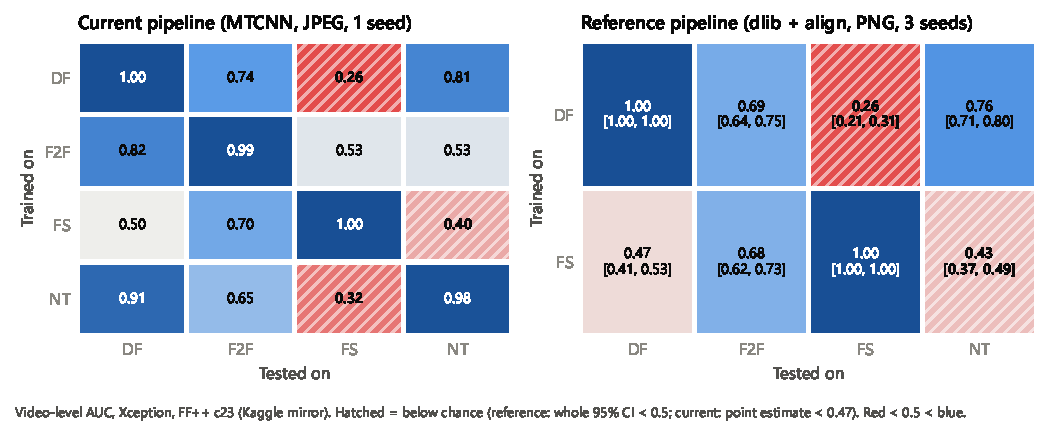
\includegraphics[width=0.92\textwidth]{F1_transfer_matrices.pdf}
\caption{Cross-manipulation video AUC for Xception. Left: original pipeline,
one seed. Right: reference pipeline, three seeds (mean and 95\% CI). Rows:
training method; columns: test method. Hatched cells are below chance.}
\label{fig:matrices}
\end{figure*}

\begin{table}[t]
\centering
\caption{One-factor preprocessing grid (Xception, 2 seeds; reference
pipeline otherwise). AUC, mean over seeds.}
\label{tab:grid}
\begin{tabular}{lccc}
\toprule
Variant & \tr{\DF}{\FS} & \tr{\FS}{\NT} & \tr{\DF}{\DF} \\
\midrule
Reference (3 seeds) & \refdffs & \reffsnt & \refdfdf \\
JPEG q95 & \pending & \pending & \pending \\
JPEG q75 & \pending & \pending & \pending \\
10 frames/video & \pending & \pending & \pending \\
Tight 1.0$\times$ margin & \pending & \pending & \pending \\
\bottomrule
\end{tabular}
\end{table}

\subsection{Mechanism: high-frequency energy}
\label{sec:mech}
High-frequency energy is the only statistic whose shift separates \FS\ from
\DF\ and \NT\ with every CI excluding zero, in both crop sets
(Fig.~\ref{fig:hf}): \DF\ $d=\hfcurdf$~\hfcurdfci, \NT\ $\hfcurnt$~\hfcurntci,
\FS\ $+\hfcurfs$~\hfcurfsci, \FF\ $\hfcurff$~\hfcurffci in the original
crops, with the same pattern in the reference crops. Comparing each fake to
the real video it was made from strengthens it (paired $d$: \DF\
\hfcurdfpaired, \NT\ \hfcurntpaired, \FS\ $+\hfcurfspaired$). \DF\ and \NT\
fakes are blurrier than real faces and \FS\ fakes are sharper.

The sign test predicts the transfer matrices (Fig.~\ref{fig:sign}): Spearman
$\rho=\sprhoxc$ for Xception and $\rho=\sprhovit$ for the hybrid, each the
best of the 24 relabelings ($p=\sppxc$), and $\rho=\sprhoref$ on the
reference matrix. It mislabels only the \FF$\leftrightarrow$\FS\ cells,
where $d_{\FF}\approx0$ carries no sign; the continuous score handles them.
Correlated sharpness statistics (Laplacian variance, noise residual) predict
nearly as well, but their \FS\ shift is close to zero.

Two checks argue that detectors use this cue rather than merely co-varying
with it. First, on real test faces alone, the \DF-trained model's fake
probability rises as faces get blurrier (Laplacian variance $\rho=\rellapdf$, $p=\relplapdf$;
noise residual $\rho=\relnoisedf$, $p=\relpnoisedf$),
the direction \DF's training fakes moved; the \FS-trained model shows no
significant reliance on high-frequency statistics. Second, the effect sizes
measured on our mirror crops predict the Xception matrix published by Li et
al.\ \cite{li2020facexray} on official data with $\rho=\pubrho$ (best of 24
relabelings, $p=\pubp$).

\begin{figure}[t]
\centering
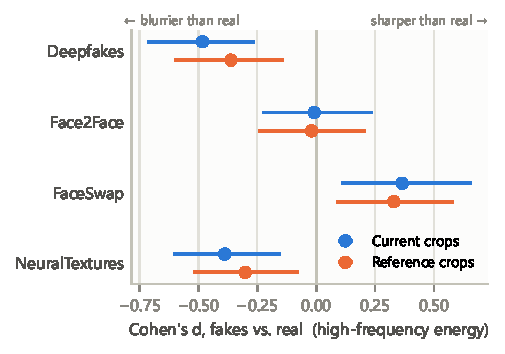
\includegraphics[width=\columnwidth]{F3_hf_effect_sizes.pdf}
\caption{High-frequency energy, fakes versus real (Cohen's $d$, 95\% CI).}
\label{fig:hf}
\end{figure}

\begin{figure}[t]
\centering
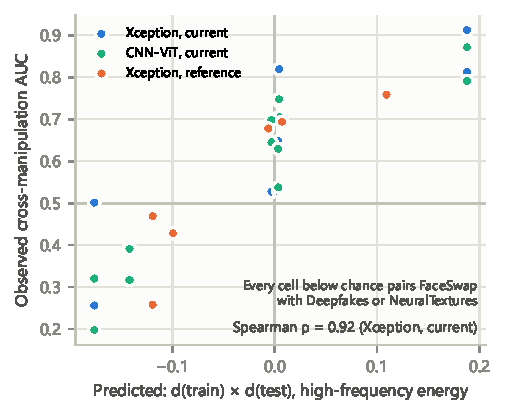
\includegraphics[width=\columnwidth]{F4_sign_prediction.pdf}
\caption{Predicted $d_A d_B$ against observed cross-manipulation AUC.}
\label{fig:sign}
\end{figure}

\subsection{Intervention}
If high-frequency energy drives the inversion, removing it as a usable cue
should reduce it. We train with label-independent random Gaussian blur or
unsharp masking (probability 0.9), which moves the \DF-versus-real effect size
on training crops from \augdfbefore\ to \augdfafter\ and \FS\ from
\augfsbefore\ to \augfsafter. Because the augmentation removes the \DF\ cue
but only weakens the \FS\ one, we predicted beforehand that \tr{\DF}{\FS}
would recover more than \tr{\FS}{\NT}. Table~\ref{tab:aug} gives the result,
with paired bootstrap CIs on the change over the same test videos.

Every cell that pairs \FS\ with \DF\ or \NT\ rises by about 0.1 AUC
(\tr{\DF}{\FS} \augdeltadffs~\augdeltadffsci, \tr{\FS}{\NT}
\augdeltafsnt~\augdeltafsntci, \tr{\FS}{\DF} \augdeltafsdf~\augdeltafsdfci)
with no in-domain cost. Both below-chance cells meet the success criterion we
set in advance (CI excluding the reference mean): \tr{\FS}{\NT} is no longer
below chance, but \tr{\DF}{\FS} remains inverted at \augaucdffs~\augaucdffsci.
Our directional prediction failed: the two cells recovered by the same
amount. The augmentation is not free either: \tr{\FS}{\FF} drops by
\augdeltafsff~\augdeltafsffci, suggesting that a \FS\ detector denied the
sharpness cue falls back on cues that transfer less well to \FF. We read
this as high-frequency energy being a substantial, causal but partial
contributor to the inversion.

\begin{table}[t]
\centering
\caption{Blur/sharpen randomization (3 seeds) versus the reference
pipeline. $\Delta$: paired change with 95\% CI.}
\label{tab:aug}
\begin{tabular}{lccc}
\toprule
Cell & Reference & Augmented & $\Delta$ \\
\midrule
\tr{\DF}{\FS} & \refdffs & \augaucdffs & \augdeltadffs~\augdeltadffsci \\
\tr{\FS}{\NT} & \reffsnt & \augaucfsnt & \augdeltafsnt~\augdeltafsntci \\
\tr{\FS}{\DF} & \reffsdf & \augaucfsdf & \augdeltafsdf~\augdeltafsdfci \\
\tr{\DF}{\FF} & \refdfff & \augaucdfff & \augdeltadfff \\
\tr{\FS}{\FF} & \reffsff & \augaucfsff & \augdeltafsff~\augdeltafsffci \\
\tr{\DF}{\DF} & \refdfdf & \augaucdfdf & \augdeltadfdf \\
\tr{\FS}{\FS} & \reffsfs & \augaucfsfs & \augdeltafsfs \\
\bottomrule
\end{tabular}
\end{table}

\begin{figure}[t]
\centering
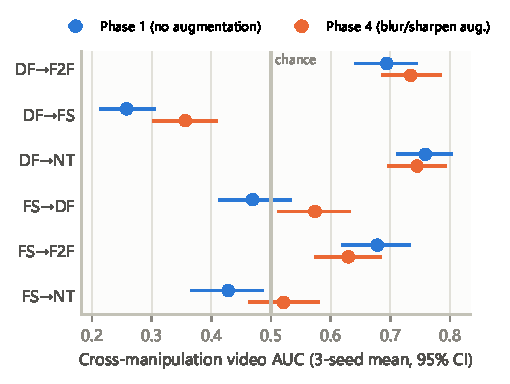
\includegraphics[width=\columnwidth]{F5_intervention.pdf}
\caption{Off-diagonal AUC with and without blur/sharpen randomization.}
\label{fig:aug}
\end{figure}

\subsection{Architectures}
If the inversion comes from a property of the training fakes rather than of
the network, other backbones should show it too. Table~\ref{tab:arch} repeats
the reference-pipeline experiment with ImageNet-pretrained ResNet-50 and
EfficientNet-B4 at the same 299\,px input as Xception (EfficientNet-B4 at
batch 16, the largest that fits in 6\,GB). ResNet-50 reproduces Xception's
below/at/above-chance call in \archrnsamecalls\ cells, including
\tr{\DF}{\FS} at \archrndffs~\archrndffsci\ and \tr{\FS}{\NT} at
\archrnfsnt~\archrnfsntci; EfficientNet-B4 matches in \archensamecalls.

\begin{figure}[t]
\centering
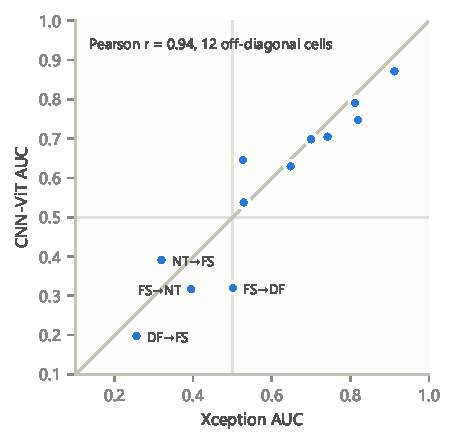
\includegraphics[width=0.85\columnwidth]{F6_architecture_agreement.pdf}
\caption{Xception versus CNN-ViT transfer AUC (original pipeline).}
\label{fig:arch}
\end{figure}

\begin{table}[t]
\centering
\caption{Backbones on the reference pipeline (2 seeds; Xception 3).}
\label{tab:arch}
\begin{tabular}{lccc}
\toprule
Backbone & \tr{\DF}{\FS} & \tr{\FS}{\NT} & \tr{\DF}{\DF} \\
\midrule
Xception & \refdffs & \reffsnt & \refdfdf \\
ResNet-50 & \archrndffs & \archrnfsnt & \archrndfdf \\
EfficientNet-B4 & \archendffs & \archenfsnt & \archendfdf \\
\bottomrule
\end{tabular}
\end{table}

\subsection{Out-of-dataset check}
On DeepFakeFace \cite{song2023dff} (IMDB-WIKI reals; SD inpainting,
InsightFace swaps and SD text-to-image fakes), we apply the same crops, measure
$d$ per generator, and evaluate the FF++-trained detectors without retraining
(1000 images sampled per class; dlib found a face in 64--90\% of them).
All three generators are blurrier than DeepFakeFace's real images
($d=\dffdinp$, \dffdins, \dffdtxt), so the sign test predicts that
\DF-trained detectors transfer and \FS-trained detectors invert on all three.
It does not hold up (Table~\ref{tab:dff}): the prediction is right on
\dffcorrect\ cells whose CI excludes chance, no better than a coin. SD
text-to-image fakes score below chance for \emph{every} detector, whatever the
sign of its training cue. Across datasets, then, something other than
high-frequency energy dominates; one candidate is that DeepFakeFace's real
images (still photographs from IMDB-WIKI) are themselves out of distribution
for detectors trained on YouTube video frames. The high-frequency account is
a within-FF++ explanation.

\begin{table}[t]
\centering
\caption{FF++-trained Xception (reference pipeline, 3 seeds) on DeepFakeFace.
AUC with 95\% CI; real class: IMDB-WIKI.}
\label{tab:dff}
\begin{tabular}{lcc}
\toprule
Generator & \DF-trained & \FS-trained \\
\midrule
SD inpainting & \dffaucdfinp~\dffaucdfinpci & \dffaucfsinp~\dffaucfsinpci \\
InsightFace & \dffaucdfins~\dffaucdfinsci & \dffaucfsins~\dffaucfsinsci \\
SD text-to-image & \dffaucdftxt~\dffaucdftxtci & \dffaucfstxt~\dffaucfstxtci \\
\midrule
Predicted & transfers & inverts \\
\bottomrule
\end{tabular}
\end{table}

\section{Limitations}
\label{sec:limits}
All FF++ results use an unofficial mirror; the agreement with published
official-data results (Sec.~\ref{sec:mech}) mitigates but does not remove this. The
sign test has only four methods, so its permutation $p$ cannot fall below
$1/24$; we tested nine statistics, and the high-frequency statistics are
correlated, so the mechanism is a well-supported candidate rather than a
proof. Phase-1 and later models use 3 or 2 seeds; the original-pipeline
matrices are single-seed point estimates. The architecture comparison in the
original pipeline is confounded by pretraining and input size (the hybrid is
trained from scratch at 224\,px). Experiments ran on one 6\,GB laptop GPU,
which bounded the preprocessing grid to factors derivable from existing
crops; detector and alignment were varied only jointly. On DeepFakeFace,
face detection succeeded at different rates per class (64--90\%), which may
bias which images enter the evaluation.

\section{Conclusion}
Below-chance cross-manipulation scores on FF++ are not noise or a
preprocessing artifact: they follow the sign of a measurable high-frequency
shift that differs between manipulation methods, a shift that predicts both
our and published transfer matrices. The shift does not predict transfer to
another dataset, where other differences dominate, so the account should be
read as within-benchmark. Detectors should be checked for such
signed shortcut cues before their cross-method scores are interpreted, and
augmentation that randomizes the cue is a cheap partial fix.

\section*{Data statement}
FF++ is not redistributed; crops, checkpoints and per-video scores stay local.
DeepFakeFace is used under its OpenRAIL licence with IMDB-WIKI-derived reals
for research only. Code and all result tables are in the project repository.

\bibliographystyle{IEEEtran}
\bibliography{refs}

\end{document}
